\begin{figure}
    \begin{center}
    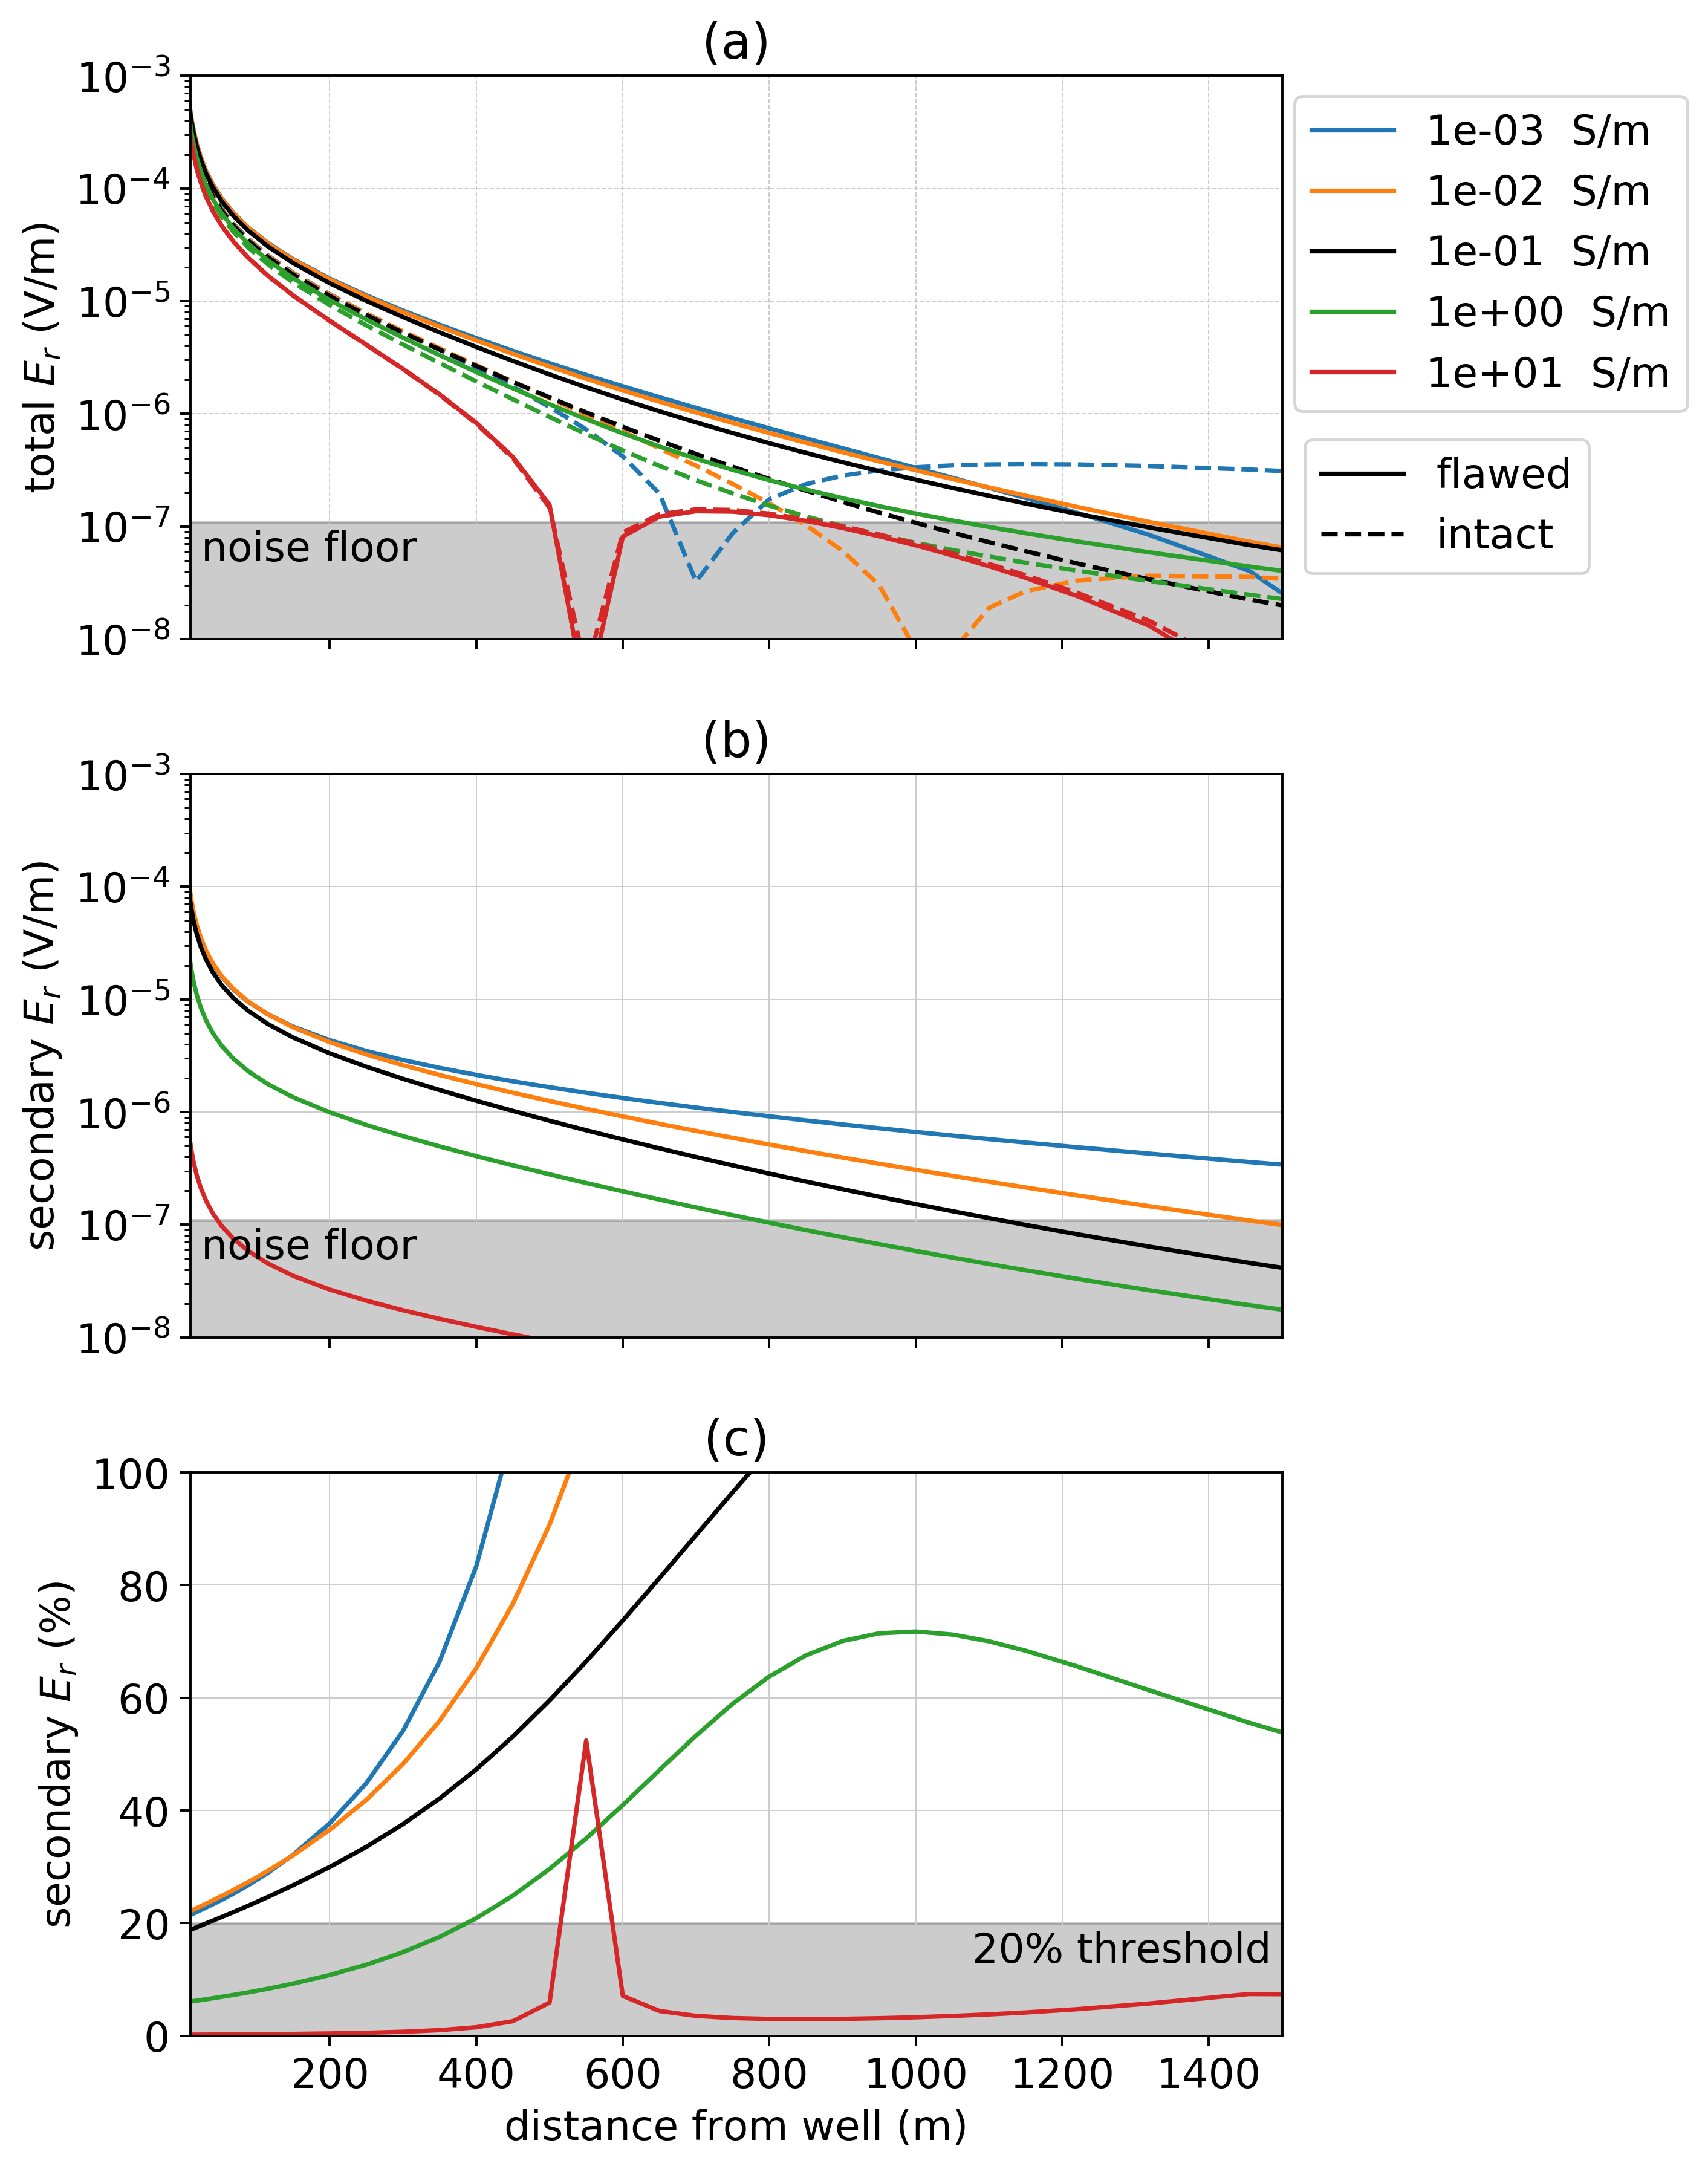
\includegraphics[width=0.8\textwidth]{figures/dc_casing/integrity_layer.png}
    \end{center}
\caption{
    Radial electric field as the conductivity of a 50m thick layer positioned at 400m depth is varied.
    The positive electrode is connected to the top of the casing, the negative electrode
    is positioned 500m away and data are measured along a line $90^\circ$ from the
    source electrodes. In (a), we show the total electric field five different layer conductivities.
    The black line shows the scenario where the layer has the same conductivity as the background.
    The dashed-lines indicate the intact well and the solid lines indicate the flawed well.
    In (b), the secondary radial electric field is plotted (with respect to an intact well primary)
    and in (c), we show the
    secondary radial electric field as a percentage of the primary.
}
\label{fig:integrity_layer}
\end{figure}
